\section{Synthesis methods and experimental conditions compared}
\label{sec:condition-matrix}

This section first summarizes what earlier experiments have established and then compares the synthesis methods according to the phase-formation process that dominates each. The tables list, item by item, the starting materials and ratios, thermal history, atmosphere and system, container and flux, cooling or growth program, and product characterization. The aim is not to assemble a recommended recipe from these entries but to keep the differences between the systems studied in view. The direct literature on the target phase establishes only an open-system high-temperature solution method and a single-crystal X-ray structure determination; the charge, temperature program, crucible, flux and cooling program are not explicitly recorded and are entered as not reported~\cite{ababaikeri2024ba5y12zn}.

\subsection{What earlier experiments established}

Three conclusions follow from the existing experiments. First, composition coordinates account for the differences in phase formation in the Ba--Y--Si--O system better than a single maximum temperature does: the Y$_2$O$_3$\slash SiO$_2$ ratio, the amount of MoO$_3$ and the cooling rate together influence the structure type and the crystal quality~\cite{kolitsch2009crystal,wierzbickawieczorek2017high}. Second, a single-crystal structure does not establish bulk phase purity; the Zn-free ceramic studies still detected secondary phases~\cite{yamane2024microstructure,gulay2024navigation}. Third, a local phase diagram turns a reproduction problem into a testable phase-region problem and gives a basis for the next round of charges~\cite{gulay2024navigation}. With this in mind, the experimental conditions of each route are compared below without rewriting the results of these related systems as a recipe for the target phase.

\subsection{Synthesis conditions on a common footing}

Figure~\ref{fig:route-matrix} organizes the literature records into three tiers: synthesis method, experimental conditions and product characterization. For the external-flux and self-flux/melt routes it lists the flux proportion, container contact, cooling and separation, melt homogenization and nucleation conditions; for the solid-state ceramic route, the mixing, pelletizing, calcination, regrinding and refiring conditions; the mechanochemical route appears only where the source explicitly reports mechanical activation; and the Czochralski route adds the seed, pulling, rotation and annealing conditions. The connecting lines mark which experimental conditions correspond to which characterization results; they do not imply that any one variable necessarily produces a particular phase.

\begin{figure*}[t]
  \centering
  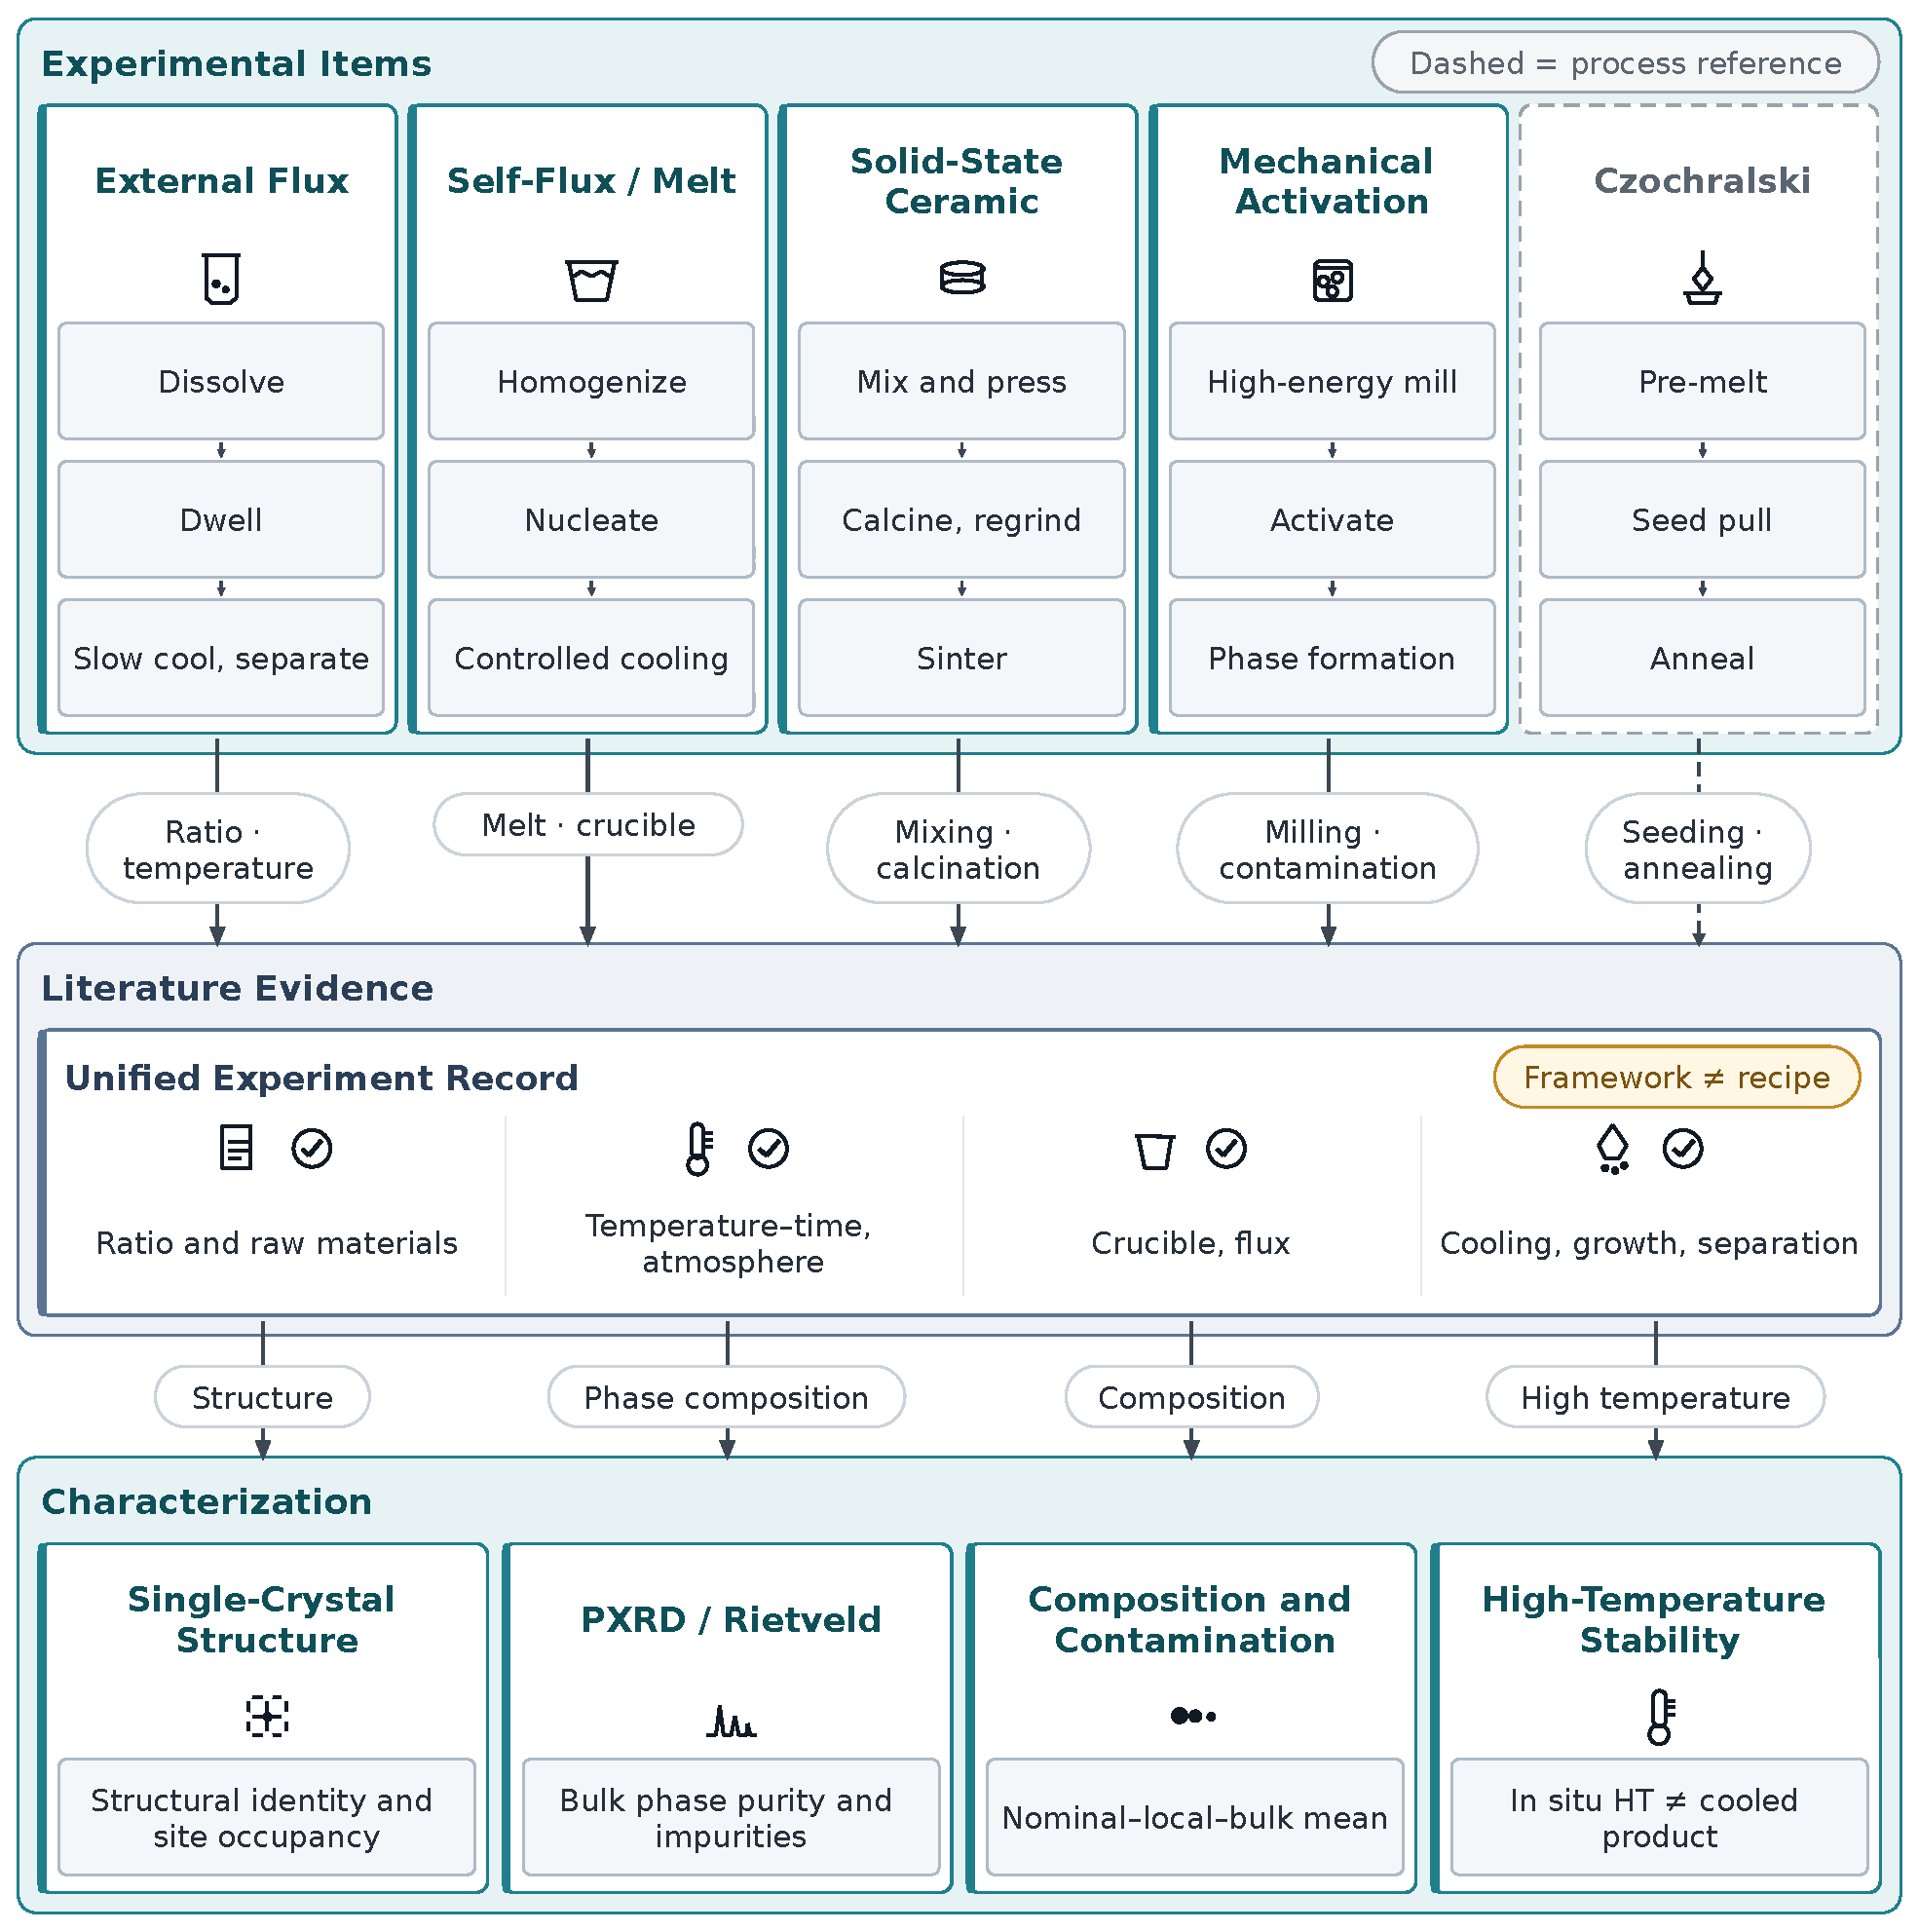
\includegraphics[width=\textwidth]{../figures/pdf/fig02_route_variable_matrix_en.pdf}
  \caption{\textbf{Conditions and product characterization compared across synthesis methods.} Left: the external-flux, self-flux/melt, solid-state ceramic, mechanochemical pre-activation and Czochralski routes. Center: the comparable starting-material, thermal-history, atmosphere, container, cooling and growth conditions. Right: complementary characterization, including single-crystal structure, PXRD\slash Rietveld refinement, compositional analysis and high-temperature stability. The connecting lines mark the correspondence between experimental conditions and characterization results, not a causal link between a variable and phase formation; the Czochralski route is included only as a process reference, and the figure is not an experimental recipe for the target phase.}
  \label{fig:route-matrix}
\end{figure*}

The number of publications behind a method says nothing about how completely its conditions are recorded. Routes such as crucible-free melt growth, open-system high-temperature solution growth or high-temperature crystallization of rare-earth silicates can be confirmed only where the source states them explicitly~\cite{christensen1994investigation,ababaikeri2024ba3zn4si4o15,leonyuk1999high,giess1982zn2sio4}. A second, title-level record by Leonyuk confirms only the single-crystal object and the structure refinement; the growth method cannot be inferred from it~\cite{leonyuk1999crystal}. The solid-state reaction literature spans structural phase transitions, ceramic sintering, dopant characterization and glass crystallization, but only items that can be traced to an experimental passage enter the numerical tables~\cite{lin1999phase,zou2021crystal,kerstan2012thermal,cai2024optimized,zhao2026crystal,tejas2024structural,pires2001luminescence,kerstan2015kristallphasen}. Among the mechanochemical sources, Tzvetkov and Minkova explicitly report mechanical treatment, whereas Yıldırım reports only additive-assisted solid--liquid-phase sintering, which does not become mechanochemical simply because the material studied is a powder~\cite{tzvetkov2001effects,yldrm2009y2sio5}. The Czochralski sources likewise serve only as process references for Y$_2$SiO$_5$\slash Ln$_2$SiO$_5$~\cite{pang2005study,alizadeh2021spectroscopy,shoudu1999czochralski,brandle1986czochralski}.

\subsection{Condition summary tables}

Table~\ref{tab:synthesis-conditions} gives each record in one row: its literature source, chemical input, synthesis method and relation to the target phase. Table~\ref{tab:synthesis-conditions-b} continues under the same numbering with the thermal history, atmosphere and system, crucible and flux, cooling or growth program, product characterization and items not recorded. Where the source column says ``experimental section'', the original experimental passage was checked; where it says ``abstract'' or ``title'', only the object or method stated there is confirmed, and steps that are not written out are not inferred from generic terms such as ``crystal growth''. A dash (``—''), or ``not reported'' within a cell, means that this check found no explicit record of the item, not that the original experiment lacked the step.

% >>> condition-matrix (generated by tools/zh_table_merge.py)
\Needspace{8\baselineskip}
{\fontsize{8}{9.8}\selectfont\setlength{\tabcolsep}{3pt}\renewcommand{\arraystretch}{1.05}
\begin{longtable}{P{\dimexpr 0.0748\textwidth-2\tabcolsep\relax}P{\dimexpr 0.1680\textwidth-2\tabcolsep\relax}P{\dimexpr 0.2157\textwidth-2\tabcolsep\relax}P{\dimexpr 0.3037\textwidth-2\tabcolsep\relax}P{\dimexpr 0.2378\textwidth-2\tabcolsep\relax}}
\caption{\textbf{Summary of synthesis conditions for the target compound and related systems (I): literature source, chemical input, synthesis method and relation to the target phase.} One row per record. Zone A holds the direct literature on the target compound; zone B the Zn-free tetragonal Ba--Y silicates of the same family, which are not reproductions of the target phase; and zone C structurally related compounds and process-reference studies. ``—'' and ``not reported'' mean that no explicit record was obtained in this check, not that the original experiment lacked the step; values for related systems are not validated recipes for the target phase.}\label{tab:synthesis-conditions}\\
\toprule
\thead{No.} & \thead{Source and location} & \thead{Target\slash product formula} & \thead{Starting materials, ratio and pretreatment} & \thead{Method; relation to target phase}\\
\midrule
\endfirsthead
\caption[]{Summary of synthesis conditions (I), continued}\\
\toprule
\thead{No.} & \thead{Source and location} & \thead{Target\slash product formula} & \thead{Starting materials, ratio and pretreatment} & \thead{Method; relation to target phase}\\
\midrule
\endhead
\midrule
\multicolumn{5}{r}{Continued on next page}\\
\endfoot
\bottomrule
\endlastfoot
\multicolumn{5}{l}{\textbf{Zone A: direct literature on the target compound}}\\*[2pt]
A1 & Publisher abstract; ESI used only to verify structure/\allowbreak{}composition~\cite{ababaikeri2024ba5y12zn} & Ba$_5$Y$_{12}$Zn[O(SiO$_4$)]$_8$ & — & High-temperature solution; external/\allowbreak{}self-flux unclear; direct report of the target compound\\
\midrule
\multicolumn{5}{l}{\textbf{Zone B: Zn-free tetragonal Ba--Y silicates of the same family; not reproductions of the target phase}}\\*[2pt]
B1 & p.~422, experimental section (accompanying-phase batch)~\cite{kolitsch2009crystal} & Ba$_{5+x}$Y$_{13}$Si$_8$O$_{41}$ (accompanying phase) & Whole batch: 1\,g each of BaCO$_3$/\allowbreak{}K$_2$CO$_3$/\allowbreak{}MoO$_3$, 0.1614\,g Y$_2$O$_3$, 0.1718\,g SiO$_2$; no stoichiometric ratio for the accompanying phase can be derived & External flux; same-family tetragonal Ba--Y silicate\\ \addlinespace[3pt]
B2 & Abstract and description of the systematic study; single-batch SI not obtained~\cite{wierzbickawieczorek2017high} & Ba$_{5+x}$Y$_{13}$Si$_8$O$_{41}$ (one phase among 151 screening runs) & BaO--K$_2$O--Y$_2$O$_3$--SiO$_2$--MoO$_3$ system; reagent form, single-batch ratio and pretreatment not reported & External flux; same-family tetragonal Ba--Y silicate\\ \addlinespace[3pt]
B3 & Process excerpt from the original (self-flux crystals)~\cite{yamane2024synthesis} & Ba$_x$Y$_{26}$Si$_{16}$O$_{71+x}$ ($x\approx10.2$) & — & Self-flux/\allowbreak{}melt; same-family tetragonal Ba--Y silicate\\ \addlinespace[3pt]
B4 & Abstract-level evidence ($9\le x\le 11$ ceramic series)~\cite{yamane2024synthesis} & Ba$_x$Y$_{26}$Si$_{16}$O$_{71+x}$ (series) & — & Solid-state ceramic; same-family tetragonal Ba--Y silicate\\ \addlinespace[3pt]
B5 & p.~598, \S2~\cite{yamane2024microstructure} & Ba$_x$Y$_{26}$Si$_{16}$O$_{71+x}$ ($9\le x\le 14$ series) & BaCO$_3$/\allowbreak{}Y$_2$O$_3$/\allowbreak{}SiO$_2$, Ba:\allowbreak{}Y:\allowbreak{}Si=$x$:\allowbreak{}26:\allowbreak{}16 ($9.0\le x\le 14.0$); starting materials heat-treated beforehand; dry-milled in an agate jar/\allowbreak{}balls at 400\,rpm for 1\,h, re-milled for 1\,h after calcination & Solid-state ceramic; same-family tetragonal Ba--Y silicate\\ \addlinespace[3pt]
B6 & Main text \S2.1.1; SI \S1.1/\allowbreak{}\S1.3~\cite{gulay2024navigation} & Ba$_5$Y$_{13}$[SiO$_4$]$_8$O$_{8.5}$ (phase A) & BaCO$_3$/\allowbreak{}Y$_2$O$_3$/\allowbreak{}SiO$_2$, BaCO$_3$:\allowbreak{}YO$_{1.5}$:\allowbreak{}SiO$_2=5{:}13{:}8$, final charge 0.5\,g; dried/\allowbreak{}preheated, ground in agate, pressed into 10\,mm pellets & Solid-state ceramic/\allowbreak{}powder; same-family tetragonal Ba--Y silicate\\
\midrule
\multicolumn{5}{l}{\textbf{Zone C: structurally related and process-reference studies --- high-temperature solution and melt}}\\*[2pt]
C1 & Publisher abstract~\cite{ababaikeri2024ba3zn4si4o15} & Ba$_3$Zn$_4$Si$_4$O$_{15}$ & — & High-temperature solution; external/\allowbreak{}self-flux unclear; structurally related compound\\ \addlinespace[3pt]
C2 & Experimental section of the IUCr original~\cite{redhammer2003beta} & $\beta$-Y$_2$Si$_2$O$_7$, with Na$_2$Si$_2$O$_5$ and oxyapatite & Na$_2$CO$_3$/\allowbreak{}Y$_2$O$_3$/\allowbreak{}SiO$_2$ in NaYSi$_2$O$_6$ proportions; nutrient:\allowbreak{}Na$_2$MoO$_4=1{:}10$; pretreatment not reported & External flux; process reference\\ \addlinespace[3pt]
C3 & Record in the original paper~\cite{giess1982zn2sio4} & Zn$_2$SiO$_4$ & Melt of $5\,$Zn$_2$SiO$_4+3\,$Pb$_2$ZnSi$_2$O$_7$; trials with a fluoride as the Zn source; pretreatment not reported & External flux; process reference\\ \addlinespace[3pt]
C4 & Title/\allowbreak{}metadata~\cite{christensen1994investigation} & High-temperature rare-earth pyrosilicates & — & Crucible-free melt; process reference\\ \addlinespace[3pt]
C5 & Indexed experimental passage of the original (flux branch)~\cite{leonyuk1999high} & Y$_2$SiO$_5$/\allowbreak{}Y$_2$Si$_2$O$_7$/\allowbreak{}LaBSiO$_5$ & Y--Si--O nutrient; Li/\allowbreak{}K di- and trimolybdates; exact ratio and pretreatment not reported & External flux; process reference\\ \addlinespace[3pt]
C6 & Title and DOI metadata~\cite{leonyuk1999crystal} & Y$_2$SiO$_5$/\allowbreak{}Y$_2$Si$_2$O$_7$/\allowbreak{}LaBSiO$_5$ & — & Unclear (title does not identify the growth route); process reference\\
\midrule
\multicolumn{5}{l}{\textbf{Zone C: structurally related and process-reference studies --- solid-state ceramic, first group}}\\*[2pt]
C7 & Experimental section of the original~\cite{lin1999phase} & BaZn$_2$Si$_2$O$_7$ & BaCO$_3$/\allowbreak{}ZnO/\allowbreak{}SiO$_2$, stoichiometric; thoroughly mixed, with intermediate grinding & Solid-state ceramic; structurally related compound\\ \addlinespace[3pt]
C8 & Experimental section of the original PDF~\cite{zou2021crystal} & BaZnSi$_3$O$_8$ & BaCO$_3$ (99.8\%), ZnO/\allowbreak{}SiO$_2$ (99.5\%); ratio not reported; ball-milled for 5\,h in a polyethylene jar/\allowbreak{}ZrO$_2$ balls/\allowbreak{}deionized water, dried at 85\,$^\circ$C, pressed at 150\,MPa & Solid-state ceramic; structurally related compound\\ \addlinespace[3pt]
C9 & Experimental section of the original; batch-to-sample mapping not disclosed~\cite{kerstan2012thermal} & Ba$_2$ZnSi$_2$O$_7$/\allowbreak{}BaZnSiO$_4$; BaZn$_{2-x}$Mg$_x$Si$_2$O$_7$ series & SiO$_2$/\allowbreak{}BaCO$_3$/\allowbreak{}ZnO; Mg from a carbonate--hydroxide hydrate; ball-milled; single-batch ratio/\allowbreak{}milling parameters not reported & Solid-state ceramic; process reference\\ \addlinespace[3pt]
C10 & Title/\allowbreak{}metadata~\cite{cai2024optimized} & BaZnSi$_3$O$_8$-based ceramics & — & Solid-state ceramic; process reference\\ \addlinespace[3pt]
C11 & Title/\allowbreak{}metadata~\cite{zhao2026crystal} & Ba$_2$MgSi$_2$O$_7$ ceramics & — & Solid-state ceramic; process reference\\
\midrule
\multicolumn{5}{l}{\textbf{Zone C: structurally related and process-reference studies --- solid-state ceramic, second group}}\\*[2pt]
C12 & Experimental section of the open-access original~\cite{tejas2024structural} & Ba$_2$ZnSi$_2$O$_7$:\allowbreak{}Sm$^{3+}$ & BaCO$_3$/\allowbreak{}ZnO/\allowbreak{}SiO$_2$ (99\%), Sm$_2$O$_3$ (99.9\%); nominal dopant ratio not reported; ground for 1\,h in an agate mortar under ethanol & Solid-state ceramic; process reference\\ \addlinespace[3pt]
C13 & Original abstract~\cite{pires2001luminescence} & Ba/\allowbreak{}Zn orthosilicates:\allowbreak{}Eu$^{3+}$/\allowbreak{}Mn$^{2+}$ & Oxides/\allowbreak{}carbonates, or Ba$_2$SiO$_4$:\allowbreak{}Eu and Zn$_2$SiO$_4$:\allowbreak{}Mn precursors; ratio and pretreatment not reported & Solid-state reaction; process reference\\ \addlinespace[3pt]
C14 & Thesis metadata/\allowbreak{}process index~\cite{kerstan2015kristallphasen} & Ba--Zn--Si crystalline phases/\allowbreak{}crystallized phases of high-temperature glass solders & — & Solid-state ceramic (glass-crystallization context); process reference\\ \addlinespace[3pt]
C15 & Institutional repository abstract~\cite{yldrm2009y2sio5} & Y$_2$SiO$_5$ powder & LiYO$_2$ additive; ratio and pretreatment not reported & Solid--liquid-phase sintering (not evidence of mechanochemical processing); process reference\\ \addlinespace[3pt]
C16 & Indexed experimental section of the original~\cite{zou2019anti} & Ba$_2$ZnSi$_2$O$_7$ & BaCO$_3$ (99.8\%), ZnO/\allowbreak{}SiO$_2$ (99.5\%); ratio not reported; ball-milled for 5\,h in a polyethylene jar/\allowbreak{}ZrO$_2$ balls/\allowbreak{}deionized water & Solid-state ceramic; process reference\\
\midrule
\multicolumn{5}{l}{\textbf{Zone C: mechanical activation and Czochralski process references}}\\*[2pt]
C17 & p.~126, \S2~\cite{tzvetkov2001effects} & Y$_2$SiO$_5$/\allowbreak{}Y$_2$Si$_2$O$_7$/\allowbreak{}yttrium oxyapatite, mixed phases & Y$_2$O$_3$/\allowbreak{}SiO$_2=7{:}9$; hydrated yttria also compared; 80\,cm$^3$ agate jar, 20\,mm agate balls/\allowbreak{}40\,g total, ball-to-powder ratio 7:\allowbreak{}1; in air at 256\,rpm for 1--3\,h & Mechanochemical pre-activation followed by heat treatment; process reference\\ \addlinespace[3pt]
C18 & Experimental section of the original~\cite{pang2005study} & Y$_2$SiO$_5$ & Y$_2$O$_3$ (99.999\%)/\allowbreak{}SiO$_2$ (99.99\%), about 980\,g, stoichiometric; mixed and ground in a corundum mortar, hydraulically pressed into blocks and prefired & Czochralski; process reference\\ \addlinespace[3pt]
C19 & Indexed experimental passage of the original (Czochralski branch)~\cite{leonyuk1999high} & Y$_2$SiO$_5$ (including a Cr-doped series) & High-purity Y$_2$O$_3$/\allowbreak{}SiO$_2$; exact ratio and prefiring not reported & Czochralski; process reference\\ \addlinespace[3pt]
C20 & Index of the growth chapter of the thesis~\cite{alizadeh2021spectroscopy} & Rare-earth-doped Y$_2$SiO$_5$ & — & Czochralski (chapter-level index); process reference\\ \addlinespace[3pt]
C21 & Indexed experimental passage of the original~\cite{shoudu1999czochralski} & Y$_2$SiO$_5$/\allowbreak{}Eu:\allowbreak{}Y$_2$SiO$_5$ & Starting materials of $\geq99.99$\% purity; melt offset from the stoichiometric composition by at most 0.2\% to compensate for SiO$_2$ volatilization (direction not clear from the original wording); prefiring not reported & Czochralski; process reference\\ \addlinespace[3pt]
C22 & Abstract of the original route study~\cite{brandle1986czochralski} & Ln$_2$SiO$_5$ (including Y$_2$SiO$_5$) & — & Czochralski; process reference\\
\end{longtable}}
\Needspace{8\baselineskip}
{\fontsize{8}{9.8}\selectfont\setlength{\tabcolsep}{3pt}\renewcommand{\arraystretch}{1.05}
\begin{longtable}{P{\dimexpr 0.0785\textwidth-2\tabcolsep\relax}P{\dimexpr 0.2148\textwidth-2\tabcolsep\relax}P{\dimexpr 0.1847\textwidth-2\tabcolsep\relax}P{\dimexpr 0.2557\textwidth-2\tabcolsep\relax}P{\dimexpr 0.2663\textwidth-2\tabcolsep\relax}}
\caption{\textbf{Summary of synthesis conditions (II): thermal history, atmosphere and system, crucible and flux, product characterization and items not recorded.} Numbering follows Table~\ref{tab:synthesis-conditions}; the labeled sub-items within a cell (cooling/growth, crucible/flux), separated by semicolons, carry over the corresponding columns of the original table.}\label{tab:synthesis-conditions-b}\\
\toprule
\thead{No.} & \thead{Temperature and time; cooling\slash growth} & \thead{Atmosphere\slash system; crucible\slash flux} & \thead{Product and characterization} & \thead{Items not recorded}\\
\midrule
\endfirsthead
\caption[]{Summary of synthesis conditions (II), continued}\\
\toprule
\thead{No.} & \thead{Temperature and time; cooling\slash growth} & \thead{Atmosphere\slash system; crucible\slash flux} & \thead{Product and characterization} & \thead{Items not recorded}\\
\midrule
\endhead
\midrule
\multicolumn{5}{r}{Continued on next page}\\
\endfoot
\bottomrule
\endlastfoot
\multicolumn{5}{l}{\textbf{Zone A: direct literature on the target compound}}\\*[2pt]
A1 & — & Open system; gas composition not reported & Single crystals; SCXRD; yield, size and bulk phase purity not reported & Starting materials, ratio, pretreatment, temperature and time, gas, crucible, flux, cooling/\allowbreak{}separation, yield/\allowbreak{}size, phase fraction\\
\midrule
\multicolumn{5}{l}{\textbf{Zone B: Zn-free tetragonal Ba--Y silicates of the same family; not reproductions of the target phase}}\\*[2pt]
B1 & 1150\,$^\circ$C, 3\,h; cooling/growth: 2\,K\,h$^{-1}$ to 900\,$^\circ$C, then slow-cooled to room temperature with the furnace switched off & Air; open/\allowbreak{}closed unclear (crucible lidded); crucible/flux: lidded Pt crucible; MoO$_3$ 1\,g; flux phase dissolved in distilled water & Colorless prismatic accompanying crystals; tentative formula from single-crystal refinement; phase-specific yield and bulk phase fraction not reported & Stoichiometric ratio/\allowbreak{}pretreatment specific to the accompanying phase, open/closed system, phase-specific yield, phase fraction\\ \addlinespace[3pt]
B2 & — & — & Multiphase screening; SCXRD\slash PXRD\slash Rietveld\slash SEM; single-batch yield of this phase not reported & Single-batch ratio, pretreatment, temperature and time, atmosphere, crucible, flux amount, cooling, yield\\ \addlinespace[3pt]
B3 & 1600\,$^\circ$C; time not reported & — & Self-flux single crystals; SCXRD; yield, size and bulk phase fraction not reported & Starting materials, ratio, pretreatment, time, system, crucible, flux, cooling, yield/\allowbreak{}size, phase fraction\\ \addlinespace[3pt]
B4 & — & — & Ceramic composition window; respective roles of SCXRD/\allowbreak{}PXRD and phase fraction not reported & Starting materials, single-point ratio, pretreatment, entire thermal history/\allowbreak{}system/\allowbreak{}container/\allowbreak{}cooling, phase fraction\\ \addlinespace[3pt]
B5 & Calcined at 1300\,$^\circ$C for 12\,h; fired at 1600\,$^\circ$C for 2\,h; cooling/growth: furnace-cooled to room temperature after power-off & Air; open/closed not reported; crucible/flux: Pt--Rh plate; lidded alumina crucible; no external flux listed & Ceramics; PXRD; secondary phases and SiO$_2$ contamination from the agate observed; quantitative phase fraction not reported & Heating and cooling rates, open/closed system, yield/\allowbreak{}phase fraction\\ \addlinespace[3pt]
B6 & Calcined at 1273\,K for 12\,h; annealed at 1573\,K for 24\,h, with regrinding and refiring twice; neutron sample additionally homogenized at 1573\,K for 12\,h; cooling/growth: crushed and finely ground after cooling; no crystal growth & Air; heating and cooling at 5\,K\,min$^{-1}$; crucible/flux: alumina crucible; no flux listed & Powder; PXRD monitoring; EDS, cRED, synchrotron PXRD, neutron TOF; yield/\allowbreak{}quantitative phase fraction not reported & Phase-specific yield, quantitative phase fraction\\
\midrule
\multicolumn{5}{l}{\textbf{Zone C: structurally related and process-reference studies --- high-temperature solution and melt}}\\*[2pt]
C1 & — & Open to air; gas flow not reported & Single crystals; SCXRD; yield, size and phase fraction not reported & Starting materials, ratio, pretreatment, temperature and time, gas flow, crucible/\allowbreak{}flux, cooling/\allowbreak{}separation, yield/\allowbreak{}size/\allowbreak{}phase fraction\\ \addlinespace[3pt]
C2 & Slowly heated to 1473\,K (1200\,$^\circ$C), 24\,h; cooling/growth: 2\,K\,h$^{-1}$ to 673\,K (400\,$^\circ$C); subsequent cooling not reported & Atmosphere and open/\allowbreak{}closed not reported (crucible lidded); crucible/flux: lidded Pt crucible; Na$_2$MoO$_4$; flux dissolved in boiling water & Colorless cube-shaped crystals with accompanying phases; SCXRD at 100/\allowbreak{}280\,K; yield not reported & Pretreatment, atmosphere/\allowbreak{}system, subsequent cooling, yield\\ \addlinespace[3pt]
C3 & 1300\,$^\circ$C to 960\,$^\circ$C; dwell not reported; cooling/growth: 1\,$^\circ$C\,h$^{-1}$; subsequent cooling not reported & Crucible/flux: crucible not reported; Pb$_2$ZnSi$_2$O$_7$/\allowbreak{}fluoride flux; separation not reported & Hexagonal prisms several millimeters long; chemical analysis/\allowbreak{}buoyancy density, formula Zn$_{1.96}$Si$_{1.04}$O$_{4.04}$ as given in the source; yield not reported & Pretreatment, dwell, system, crucible, separation, subsequent cooling, yield\\ \addlinespace[3pt]
C4 & — & Crucible/flux: crucible-free; flux not reported & Melt product; neutron powder diffraction/\allowbreak{}profile refinement; yield and phase fraction not reported & Starting materials, ratio, pretreatment, temperature and time, system, flux, cooling, yield/\allowbreak{}phase fraction\\ \addlinespace[3pt]
C5 & — & Crucible/flux: Li/\allowbreak{}K molybdate flux; crucible, flux ratio and separation not reported & Spontaneously nucleated crystals; electron microprobe, XRD/\allowbreak{}structure refinement; yield not reported & Exact ratio, pretreatment, temperature and time, system, crucible, flux ratio/\allowbreak{}separation, cooling, yield\\ \addlinespace[3pt]
C6 & — & — & Title supports only the single-crystal object and the structure refinement; yield/\allowbreak{}size not reported & Starting materials, ratio, pretreatment, synthesis method and all experimental conditions, yield/\allowbreak{}size\\
\midrule
\multicolumn{5}{l}{\textbf{Zone C: structurally related and process-reference studies --- solid-state ceramic, first group}}\\*[2pt]
C7 & 1280\,$^\circ$C; time not reported & — & White polycrystalline powder; PXRD, neutron diffraction, GSAS/\allowbreak{}Rietveld; yield/\allowbreak{}phase fraction not reported & Time, system, crucible/\allowbreak{}flux, cooling, yield/\allowbreak{}phase fraction\\ \addlinespace[3pt]
C8 & Calcined in air at 1000\,$^\circ$C for 3\,h (5\,$^\circ$C\,min$^{-1}$); sintered at 1090--1120\,$^\circ$C for 3\,h; cooling/growth: 2\,$^\circ$C\,min$^{-1}$ to 1000\,$^\circ$C, then furnace-cooled & Air; open/\allowbreak{}closed not reported & Ceramics; laboratory/\allowbreak{}synchrotron XRD with Rietveld refinement; yield/\allowbreak{}quantitative phase fraction not reported & Ratio, open/closed system, crucible/\allowbreak{}flux, yield/\allowbreak{}phase fraction\\ \addlinespace[3pt]
C9 & Cooling/growth: ball-milled again after cooling; cooling rate not reported & — & Polycrystalline; HT-XRD, dilatometry; single-batch phase fraction not reported & Single-batch ratio/\allowbreak{}milling, temperature and time, system, crucible/\allowbreak{}flux, cooling rate, phase fraction\\ \addlinespace[3pt]
C10 & — & — & Ceramics; structural/\allowbreak{}microwave-dielectric characterization; phase-purity method and phase fraction not reported & Starting materials, ratio, pretreatment and all experimental conditions, phase fraction\\ \addlinespace[3pt]
C11 & — & — & Ceramics; structural/\allowbreak{}sintering/\allowbreak{}microwave-dielectric characterization; phase-purity method and phase fraction not reported & Starting materials, ratio, pretreatment and all experimental conditions, phase fraction\\
\midrule
\multicolumn{5}{l}{\textbf{Zone C: structurally related and process-reference studies --- solid-state ceramic, second group}}\\*[2pt]
C12 & 1200\,$^\circ$C for 6\,h in O$_2$; heated at 5\,$^\circ$C\,min$^{-1}$; cooling/growth: cooled naturally to room temperature, then ground & O$_2$; open/\allowbreak{}closed not reported; crucible/flux: alumina crucible; flux not reported & Powder; XRD/\allowbreak{}FTIR/\allowbreak{}SEM--EDS/\allowbreak{}thermal and spectroscopic analysis; yield/\allowbreak{}phase fraction not reported & Dopant ratio, open/closed system, flux, yield/\allowbreak{}phase fraction\\ \addlinespace[3pt]
C13 & — & — & Powder; PXRD/\allowbreak{}IR/\allowbreak{}UV--vis/\allowbreak{}luminescence; yield/\allowbreak{}phase fraction not reported & Ratio, pretreatment and all experimental conditions, yield/\allowbreak{}phase fraction\\ \addlinespace[3pt]
C14 & — & — & Crystallized phases; HT-XRD/\allowbreak{}dilatometry characterization index; single-batch phase fraction not reported & Starting materials, ratio, pretreatment and all single-batch experimental conditions, phase fraction\\ \addlinespace[3pt]
C15 & — & Crucible/flux: crucible not reported; LiYO$_2$ additive amount not reported & Powder; optical microscopy, XRD, SEM--EDS; yield/\allowbreak{}phase fraction not reported & Ratio, pretreatment and entire thermal history/\allowbreak{}system/\allowbreak{}container/\allowbreak{}cooling, yield/\allowbreak{}phase fraction\\ \addlinespace[3pt]
C16 & Calcined in air at 1100\,$^\circ$C for 3\,h; sintered in air/\allowbreak{}O$_2$/\allowbreak{}N$_2$ at 1200\,$^\circ$C or in N$_2$--1\,vol\% H$_2$ at 1125\,$^\circ$C; sintering time not reported & Air/\allowbreak{}O$_2$/\allowbreak{}N$_2$/\allowbreak{}N$_2$--1\,vol\% H$_2$; open/\allowbreak{}closed not reported & Ceramics; XRD/\allowbreak{}XPS/\allowbreak{}microwave dielectric; BaSiO$_3$ observed in samples sintered under reducing atmosphere; yield/\allowbreak{}phase fraction not reported & Ratio, sintering time, open/closed system, crucible/\allowbreak{}flux, cooling, yield/\allowbreak{}phase fraction\\
\midrule
\multicolumn{5}{l}{\textbf{Zone C: mechanical activation and Czochralski process references}}\\*[2pt]
C17 & Subsequent heat treatment in air for 2\,h; the abstract summarizes phase formation as $T>1000\,{}^\circ$C, and the specific set points are not fully given in this passage & Milling and heat treatment both in air; open/\allowbreak{}closed not reported; crucible/flux: agate balls/\allowbreak{}jar for milling; crucible and flux for the synthesis heat treatment not reported & Mixed-phase powder; XRD/\allowbreak{}IR/\allowbreak{}thermal analysis; phase fraction not reported & Specific temperatures of the synthesis heat treatment, open/closed system, heat-treatment crucible/\allowbreak{}flux, cooling, phase fraction\\ \addlinespace[3pt]
C18 & Single-phase charge prepared at 1200\,$^\circ$C for 24\,h; melting temperature/\allowbreak{}growth time not reported & High-purity N$_2$; open/\allowbreak{}closed not reported; crucible/flux: Ir crucible, 80$\times$60\,mm; flux not applicable & Single crystal; orientation, optical microscopy, SEM, absorption spectra; structural phase purity/\allowbreak{}yield not reported & Melting temperature/\allowbreak{}growth time, open/closed system, pulling/\allowbreak{}rotation rate/\allowbreak{}cooling, structural phase purity/\allowbreak{}yield\\ \addlinespace[3pt]
C19 & Cooling/growth: pulled at 2.0--2.5\,mm\,h$^{-1}$; rotation, cooling/\allowbreak{}annealing not reported & Crucible/flux: RF-heated Ir crucible, about 80$\times$90\,mm; flux not applicable & Large crystals/\allowbreak{}spontaneously nucleated crystals; electron microprobe, XRD/\allowbreak{}structure refinement; yield not reported & Exact ratio/\allowbreak{}prefiring, melting temperature/\allowbreak{}time, system, rotation/\allowbreak{}cooling/\allowbreak{}annealing, yield\\ \addlinespace[3pt]
C20 & — & Crucible/flux: crucible not reported; flux not applicable & Crystals/\allowbreak{}spectroscopic and crystal-field analysis; structural phase purity, yield/\allowbreak{}size not reported & Starting materials, ratio, prefiring and all growth parameters, structural phase purity/\allowbreak{}yield/\allowbreak{}size\\ \addlinespace[3pt]
C21 & Melting temperature and growth time not reported; post-growth anneal for 20\,h & Crucible/flux: RF-heated Ir crucible; flux not applicable & Crystals about 35\,mm$\times$130\,mm, 460--486\,g; Ir inclusions seen under the microscope; structural phase purity/\allowbreak{}yield not reported & Prefiring, melting temperature/\allowbreak{}growth time, system, pulling/\allowbreak{}rotation/\allowbreak{}cooling, annealing temperature, structural phase purity/\allowbreak{}yield\\ \addlinespace[3pt]
C22 & — & Crucible/flux: crucible not reported; flux not applicable & Single crystals; melt stability, dopant partitioning and facet formation studied; structural phase purity/\allowbreak{}yield not reported & Starting materials, ratio, prefiring and all growth parameters, structural phase purity/\allowbreak{}yield\\
\end{longtable}}
% <<< condition-matrix

\subsection{Comparison by zone}

The central point of zone A is that the direct literature gives no complete recipe: for the target compound, only the route category and the SCXRD result can currently be checked, and no recipe item can be back-filled from related systems~\cite{ababaikeri2024ba5y12zn}. Zone B shows that work on the Zn-free Ba--Y silicates of the same family already covers flux-grown accompanying phases, self-flux crystals, ceramic composition scans and multi-probe solid-state/powder phase-region studies, but none of it concerns the Zn-containing target phase; in particular, the systematic screening for which no single-batch SI was obtained cannot be compressed into a single ``representative condition''\cite{kolitsch2009crystal,wierzbickawieczorek2017high,yamane2024synthesis,yamane2024microstructure,gulay2024navigation}.

The direct value of zone C is that it shows how experimental conditions differ between methods. High-temperature solution papers usually report the flux composition, container and slow-cooling/separation conditions together, whereas solid-state reaction papers more often report the mixing, calcination, regrinding and sintering conditions; when the same system is prepared under different atmospheres, volatilization losses and secondary phases must also be treated as product information, and the atmosphere cannot be regarded as an isolated ``optimization variable''\cite{redhammer2003beta,zou2021crystal,zou2019anti}. C17 reports the rotation speed, duration, agate balls/jar and ball-to-powder ratio, so its mechanical activation step can be described, but the product remains a mixed-phase powder and cannot supply a recipe for the target phase; Czochralski studies, even where they report the charge, crucible and crystal size, still need structural and phase-purity characterization, and whether the target phase can be grown cannot be inferred from the appearance of a crystal~\cite{tzvetkov2001effects,pang2005study,leonyuk1999high,shoudu1999czochralski}. The values in the tables therefore hold only within their own literature records: they are not merged across publications or averaged across compounds, and ``not given in the abstract'' is never rewritten as ``not reported in the original''.
